\documentclass[12pt,a4paper]{article}
\usepackage{times}
\usepackage{durhampaper}

\usepackage{harvard}
% package to add dumptext
\usepackage[english]{babel}
\usepackage{blindtext}

% package to add wrapfigure
\usepackage{wrapfig}

% packages to add images
\usepackage{graphicx}

% packages for pseudocode and algorithms
\usepackage{amsmath}
\usepackage{algorithm}
\usepackage[noend]{algpseudocode}
\makeatletter
\def\BState{\State\hskip-\ALG@thistlm}
\makeatother

% packages to generate neural network graph
\usepackage{tikz}
\usetikzlibrary{matrix,chains,positioning,decorations.pathreplacing,arrows}

% package to add graphs
\usepackage{pgfplots}

\citationmode{abbr}
\bibliographystyle{agsm}

\title{Playing Draughts using Neural Networks and Genetic Algorithms}
\author{Thien P. Nguyen}
\student{Thien P. Nguyen}
\supervisor{Stefan Dantchev}
\degree{BSc Computer Science}

% stuff for checkerboard
\usetikzlibrary{matrix.skeleton}
\tikzstyle{ball} = [circle, shading=ball, minimum size=1cm]
\newcommand{\bl}{\node [ball, ball color=black!80!white, draw=black!65!white, thin]{};}
\newcommand{\wh}{\node [ball, ball color=white] {};}


% -------------------------------------------------------------------

\begin{document}

\maketitle

\begin{abstract}

    {\bf Background}

    Presently, competitive Draughts AI players are currently designed to play at a fixed ability. While it has produced very competitive and intelligent players, they require some human intervention to improve their performance. 
    This is due to their dependency on pre-defined move databases. Optimal moves are pre-calculated, and recalled when necessary. By combining Neural Networks and Genetic Algorithms, this issue could possibly be solved by creating a player that can grow in ability over time, without the dependency on move-banks.
    
    {\bf Aims}

    The purpose of this project is to explore approaches to tackle the game of English Draughts via the use of machine learning techniques. First, we study previous historical successes in the field, and look at the components that helped build their systems. Then, we look at contemporary methods of computer science that could be used to evolve the historical systems. The project will establish whether this approach provides an effective performance on the game.
    
    {\bf Method}

    The initial population consists of randomly generated AI players, which will play each other to determine the best player out of the population. The performance of championing AI players at every generation of the genetic algorithm are measured against previous champions. Appropriate algorithms are implemented to determine the overall development of the system's ability to play Draughts.

    {\bf Proposed Solution}.  

    The proposed solution starts with designing a feed-forward neural network that evaluates the probability of a particular side winning, given a state of a checkerboard. This is then used in a algorithm that evaluates future moves to predict the best move at a given position. This, alongside a set of weights for the neural network, creates a player that can evaluate potential moves. Finally, the player is then used on an existing Draughts framework that will provide the player with the ability to play Draughts. Genetic algorithms are used to adjust the weights of the neural network, with the intention of making the system learn to evaluate checkerboards more precisely.

\end{abstract}

\begin{keywords}
    Artificial Intelligence, Neural Networks, Genetic Algorithms, Draughts, Machine Learning, Monte Carlo Tree Search
\end{keywords}

\section{Introduction}

    The intention of this project is to explore the effectiveness of genetic algorithms to improve the neurons of a neural network. Neural networks can be used to evaluate the performance of two players in a zero-sum game of Draughts. We attempt to manipulate the neurons through the use of genetic algorithms to increase the accuracy of the evaluation. This would potentially allow us to create an effective Draughts playing agent that, when provided with the option to consider a set of moves, would have the ability to play and learn without human input.

\subsection*{Draughts}

    English Draughts (or Checkers) is a popular 2-player board-game played on an 8x8 chess board. Players choose a colour and begin with 12 pawns each of their respective colours, and they are placed on the dark-coloured squares of the board. Beginning with the black pawns, each player takes a turn to move a pawn diagonally in one square. In the event that a pawn reaches the opposite side of the board from where the piece originated, it is promoted to a king. Kings have the ability to traverse backwards in the same diagonal motion as pawns. Assuming that there is space upon landing, A piece (pawn or king) also has the option to capture their opponents piece by moving two consecutive diagonal squares, where the opponents piece is situated immediately opposing the players piece. Pieces can be captured consecutively in a single turn if the moves afford the scenario. A player wins by capturing all of their opponents pieces. A player loses by having all of their pieces captured. A draw occurs when both players agree to draw after a three-fold repetition (where both players take three moves to simulate the same position), or a player has pieces on the board but cannot move any of them. A draw can be forced when both players fail to capture a piece after a set amount of moves.

\subsection*{Genetic Algorithms}

    Genetic algorithms (GAs) are a group of search techniques used to find exact or approximate solutions to optimisation and search problems. The methodology is inspired by Charles Darwin's evolutionism theory; individuals are created by the crossover of the genetic information (genome) of their parents. Genomes are metaphors of genetic information; it typically refers to a data structure, most commonly an 1D array. Genetic Algorithms generally consist of a population of agents, a tournament selection process, algorithmic crossover mechanisms against the genomes of the agents, and the introduction of probabilistic mutation on genomes. 

\subsection*{Neural Networks}

    Neural Networks are non-linear statistical data-modelling tools, linking inputs and outputs adaptively in a learning process similar to how the human brain operates. Networks consist of units, described as neurons, and are joined by a set of rules and weights. The units are defined with characteristics, and appear in layers. The first layer is defined as the input layer, and the last layer being the output. Layers between the two aforementioned are described as hidden layers. Data is analysed through their propagation through the layers of neurons. Learning takes place in the form of the manipulation of the weights connecting the units in the layers. This allows it to model complex relationships between inputs and output, and it can also find patterns in the data. 

\subsection*{Motivation}
    % Research Question
    Whilst the use of evolutionary algorithms and neural networks have been explored to create draughts players, my intention is to explore the effectiveness of genetic algorithms and neural networks. The intention is to determine the possibility of developing a performing draughts playing agent by the use of GANNs (Genetic Algorithms and Neural Networks).

\subsection*{Deliverables}

    \subsubsection*{Minimum}

    \begin{itemize}
    \item Implement a feed-forward neural network
    \item Implement a checkers game interface
    \item Implement a decision making process that chooses a move from a given position of a checkers board.
    \item Implement a genetic algorithm that uses a population of agents that have their own independently functioning neural network.
    \end{itemize}

    \subsubsection*{Intermediate}

    \begin{itemize}
    \item An interface to play against an agent.
    \item A monte-carlo search of the move space.
    \item Multi-processing of the tournament selection process for the genetic algorithm.
    \end{itemize}

    \subsubsection*{Advanced}

    \begin{itemize}
    \item Evidence shown to indicate that the system is learning over time.
    \item An agent produced by this process can play to an ELO of at least 1200.
    \item Agents can be played against human input through a simple user interface.
    \end{itemize}

\subsection*{Related Work}

    Arthur Samuel pioneered the concept of an self learning program that can play Checkers, through the use of using evolutionary algorithms \cite{samuel_studies_2000}. However, the work described did not consider the use of neural networks (as it was not conceived at the time). It was also dependent on a set of heuristics Samuel devised. This could handicap the agent's ability to play, as they are dependent on the effectiveness of Samuel's heuristics. 

    The idea of evolving neural networks to play Draughts is based on the success Chellapilla and Fogel had in evolving their own Checkers neural networks \cite{chellapilla_evolving_1999}. Their work, Blondie24, used a neural network as the evaluator function, and used an evolutionary algorithm (most notably mutation on parents) to evolve the agents. However, crossover mechanisms were not considered (and thus not using genetic algorithms). Blondie24's neural network structure consists of a $\left\{ 32,40,10,1 \right\}$ set. Spatial awareness is not considered as it takes an immediate input of the positions on the board. This makes it inherently more difficult for the neural network to generate heuristics based on spatial awareness. Relative distance between pieces are not encapsulated in a method that can be immediately interpreted by the neural network.
    Their decision making algorithm primarily revolved around a mini-max algorithm with a ply cap. Advancements in the field led to more successful algorithms, which will be explained later on. 
    
    Lai's Giraffe \cite{lai_giraffe:_2015} program used a deep reinforcement learning technique to play Chess to an advanced level in a relatively quick time-period. Giraffe's decision function involved using Temporal Difference Learning (TD-Leaf), an improvement on MiniMax, by Baxter et al. \cite{baxter_tdleaflambda_1999} However, Giraffe has been trained on previously played games from grandmaster tournaments as a reference, and was not entirely self-taught.

% ----------------

\section{Design}

\subsection*{Algorithms and Data Structures}

\subsubsection{Decision Making Algorithm}

    To choose the best move given a current position, an initial decision making process for an agent could revolve around the use of minimax algorithm. This was the case for Chellapilla and Fogel's agent. \cite{chellapilla_evolving_1999}. This algorithm would expand a tree of potential moves. Each node represents a state of a checkerboard. Child nodes represent a state of the checkerboard for a given move. Child nodes can only be produced from the parent node; i.e a move from a parent node will produce a child node. 
    
    Child nodes are expanded until some depth is reached. From here, an evaluation function is used to calculate the value of the leaf nodes at this depth. This evaluation function produces a value that indicates a players advantage in a given state. The best potential position for a given player can be deduced from the nodes at this stage, which is quantified with a value.

    The best value propagates upwards until it reaches to a child of the root node. This represents an agent's current state of the game. The use of alpha-beta pruning would help to ignore evaluating unnecessary moves, reducing the number of calculations. Once the possible moves have been considered, the best child node is chosen, representing the best move at a given position.

    The mini-max method will have a search depth of 4ply (where the agent will search four moves ahead.) This should allow the agents to form a basic strategy where they can plan their moves in advance. There are inherent trade-offs with having a higher ply count; asymptotic complexity of mini-max is exponential; it being $O(x^y)$ for $x$ being the branching factor, and $y$ being depth. Branching factor will consist of the moves from each agent in a given game. This exponential growth is the achilles heel to the mini-max approach.

    Once initial development on the mini-max algorithm is complete, The project will migrate to a hybrid technique that combines mini-max and a more contemporary algorithmic paradigm, Monte-Carlo Tree Search (MCTS). MCTS differs from mini-max where future moves are randomly played to the end of the game. It acts as a sampling of possible outcomes, and does not depend on an evaluation function at all. The random simulation of games are skewed such that more reasonable moves are chosen. A survey by Browne et al. found that MCTS can dramatically outperform mini-max based search engines in games where evaluation functions are otherwise difficult to obtain \cite{browne_survey_2012}.

    MCTS-EPT (or MCTS with early playout termination) is introduced by Lorentz \cite{lorentz_using_2016}. MCTS-EPT modifies the MCTS random play-out approach; Instead of allowing the random moves play to the end of the game, the number of moves traversed are capped and an evaluation function can be used from that caped position instead. The termination ply would be capped at 6ply. This could potentially improve the amount of foresight for a given set of moves, without the need to depend on random generations of moves to the end, and the need to evaluate more moves (as typically needed even with alpha-beta pruning on a mini-max algorithm).

    We retain the minimax algorithm in order to evaluate the performance differences between our two decision making algorithms.
    
    \begin{figure}[ht!]
        \centering
        \caption{The chosen neural network model. The preprocessed values of the checkerboard are used as input. An output is produced after propagation that ranges from [-1,1]. \label{nnmodel}}
        \vspace{10pt}
        \tikzset{%
        every neuron/.style={
            circle,
            draw,
            minimum size=0.9cm
            },
        neuron missing/.style={
            draw=none, 
            scale=4,
            text height=0.333cm,
            execute at begin node=\color{black}$\vdots$
        },
    }

    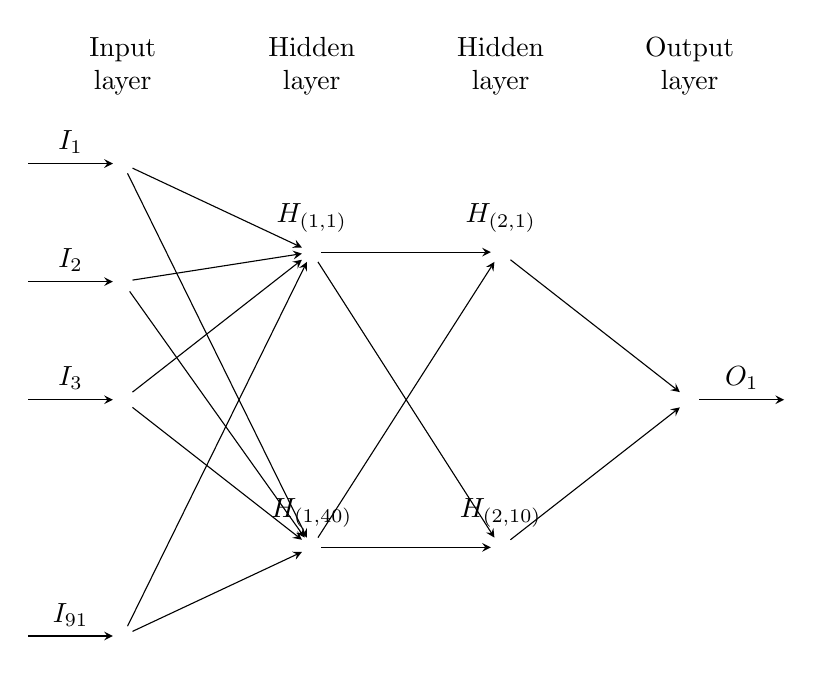
\begin{tikzpicture}[x=1.2cm, y=1.5cm, >=stealth]

    % draw nodes
        % % input values
        % \foreach \m/\l [count=\y] in {1,2,3,missing,4}
        % 	\node [every neuron/.try, neuron \m/.try] (input-\m) at (-0.5,2.5-\y) {};

        % input layer
        \foreach \m/\l [count=\y] in {1,2,3,missing,4}
        \node [every neuron/.try, neuron \m/.try] (input-\m) at (0,2.5-\y) {};
        
        % layer 1
        \foreach \m [count=\y] in {1,missing,2}
        \node [every neuron/.try, neuron \m/.try ] (hidden1-\m) at (2,2-\y*1.25) {};

        % layer 2
        \foreach \m [count=\y] in {1,missing,2}
        \node [every neuron/.try, neuron \m/.try ] (hidden2-\m) at (4,2-\y*1.25) {};

        % output layer
        \foreach \m [count=\y] in {1}
        \node [every neuron/.try, neuron \m/.try ] (output-\m) at (6,0.5-\y) {};

    % input layer
    \foreach \l [count=\i] in {1,2,3,91}
        \draw [<-] (input-\i) -- ++(-1,0)
        node [above, midway] {$I_{\l}$};

    % hidden 1
    \foreach \l [count=\i] in {{(1,1)},{(1,40)}}
        \node [above] at (hidden1-\i.north) {$H_{\l}$};

    % hidden 2
    \foreach \l [count=\i] in {(2,1),(2,10)}
        \node [above] at (hidden2-\i.north) {$H_{\l}$};

    % output layer
    \foreach \l [count=\i] in {1}
        \draw [->] (output-\i) -- ++(1,0)
        node [above, midway] {$O_\l$};

    % lines from input to hidden 1
    \foreach \i in {1,...,4}
        \foreach \j in {1,...,2}
            \draw [->] (input-\i) -- (hidden1-\j);
    
    % lines from hidden 1 to hidden 2
    \foreach \i in {1,...,2}
    \foreach \j in {1,...,2}
        \draw [->] (hidden1-\i) -- (hidden2-\j);

    % lines from hidden 2 to output
    \foreach \i in {1,...,2}
        \foreach \j in {1}
            \draw [->] (hidden2-\i) -- (output-\j);

    % headings
    \foreach \l [count=\x from 0] in {Input, Hidden, Hidden, Output}
        \node [align=center, above] at (\x*2,2) {\l \\ layer};

    \end{tikzpicture}
        % \vspace{-25pt}
    \end{figure}
 
\subsubsection{Neural Network}

    To evaluate the board, we use a feed-forward multilayer perceptron style neural network. The network would contain 4 layers; the input layer consists of 91 nodes, with the output node having 1. Hidden layers will have 40 and 10 nodes respectively. Figure \ref{nnmodel} shows the network in the form of a diagram.
    
    Common knowledge infers that a king is worth more than a pawn, but it is disputed about its precise value advantage. For the sake of simplicity, a king's piece value is to be weighted at $1.5x$ a pawn value; a value of a pawn will be $1$. 

    The input array takes in the form of the grid array of the board. The intention is to weigh the Black pawns with a value of 1, and white pawns as -1. To create the input layer, we treat the checkerboard into a 1D array, with the indexes displayed in figure \ref{boardarray}. The array is used to calculate all possible sub-squares of the checkerboard, ranging from a 3x3 kernel to a 8x8. Each sub-square is summed up to create an input node. There are consequently 91 combinations of the sub-squares, thus forming the input layer. 

    \begin{wrapfigure}{l}{0.37 \textwidth}
        % \begin{center}
        \fontsize{8}{11}
        % \vspace{-25pt}
        \centering
            \caption{The indexes of the 32 pieces of the input layer are the immediate values of the positions on the board. \label{boardarray}}
            \vspace{5pt}
            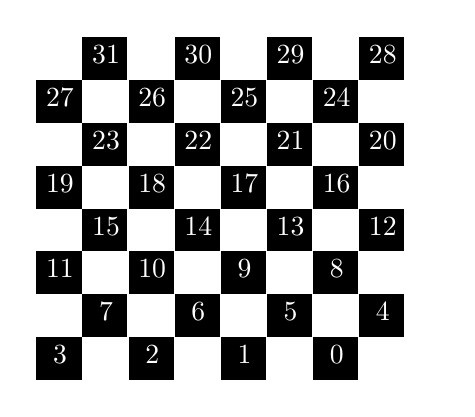
\begin{tikzpicture}
            \color{white}
            \matrix (m) [matrix of nodes, nodes in empty cells, label skeleton, nodes={minimum size = 0.4cm}] {
            & 31 &&30&&29&&28 \\
            27 &&26&&25&&24&&\\
            &23&&22&&21&&20\\   
                19&&18&&17&&16&&\\
            &15&&14&&13&&12\\
            11&&10&&9&&8&&\\
            &7&&6&&5&&4\\
            3&&2&&1&&0\\
            % \bl &     & \bl &     &     &     & \bl &     \\
            %     &     &     & \bl &     &     &     &     \\
            % \wh &     &     &     &     &     &     &     \\
            %     &     &     & \wh &     & \wh &     & \wh \\
            % \wh &     & \wh &     & \wh &     & \wh &     \\
            %     & \wh &     & \wh &     & \wh &     & \wh \\
            };
            \foreach \row in {1, ..., 8} {
            \foreach \col in {1, ..., 8} {
                \pgfmathparse{Mod(\row + \col, 2) ? "black" : "white"}
                \colorlet{squarebg}{\pgfmathresult}
                \fitandstyle[background]{(m-cell-\row-\col)}{fill = squarebg}
            }
            }
            \end{tikzpicture}
        % \end{center}
      
    \end{wrapfigure}
    
    % Talk about the activation function
    Weights of a neuron are summed with their bias, and are passed through an activation function (or transfer function) $O = f((Input* weight) + Bias)$ to become an input for another neuron. Activation functions usually have a sigmoid curve, but may also take the form of other shapes. Common characteristics of activation functions include values to be monotonically increasing, continuous, differentiable and bounded.
    % how does it work?

    Our initial choice for the activation function is tanh, shown in figure \ref{sigmoid}. There exists inherent issues related to the properties of their derivatives, discussed by Nair and Hinton \cite{nair_rectified_2010}, described as the missing gradient problem. However, since this issue is related to the properties of a gradient based learning method and not through a stochastic learning method (of which genetic algorithms are), this is not a concern for the project. Sigmoidal function also facilitates the ability to simulate a zero sum formula (for a range of -1 to 1) due to its central symmetric properties.

    \begin{wrapfigure}{r}{0.4\textwidth}
        \centering
        \vspace{-30pt}
        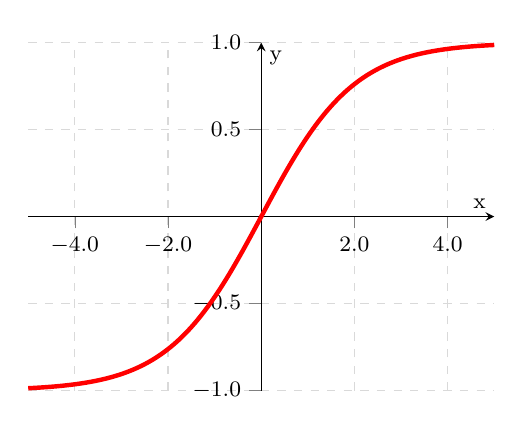
\begin{tikzpicture}
            \fontsize{8}{11}
            \begin{axis}[
                legend pos=north west,
                axis x line=middle,
                axis y line=middle,
                x tick label style={/pgf/number format/fixed,
                                    /pgf/number format/fixed zerofill,
                                    /pgf/number format/precision=1},
                y tick label style={/pgf/number format/fixed,
                                    /pgf/number format/fixed zerofill,
                                    /pgf/number format/precision=1},
                grid = major,
                width=75mm,
                height=6cm,
                grid style={dashed, gray!30},
                xmin=-5,     % start the diagram at this x-coordinate
                xmax= 5,    % end   the diagram at this x-coordinate
                ymin= -1,     % start the diagram at this y-coordinate
                ymax= 1,   % end   the diagram at this y-coordinate
                %axis background/.style={fill=white},
                xlabel=x,
                ylabel=y,
                tick align=outside,
                enlargelimits=false]
            % plot the stirling-formulae
            \addplot[domain=-5:5, red, ultra thick,samples=500] {2*(1/(1+e^-x))-1};
            % \addlegendentry{$f(x)=\frac{1}{1+e^{-5x}}$}
            \end{axis}
        \end{tikzpicture}
        \caption{Graph of tanh function $f(x)={\frac{2}{1+e^{-x}}- 1}$ (An example of an activation function with a sigmoid curve). \label{sigmoid}}
        \vspace{-30pt}
    \end{wrapfigure}

\subsubsection{Genetic Algorithms} \label{genetic_algorithms}

    The genetic algorithm is the premise of the system's learning strategy. GA's are used to train the neural network. We discuss the various algorithms that form the collection of GA strategies below. For the system, a population size of 15 is chosen.


\subsubsection{Population Generation} \label{population_generation}
    % Introduce what its for
    In genetic algorithms, the population serves as a base that allows agents in the pool to play each other. Every generation has its own population, with all having the same number of agents. The initial population will consist of randomly generated weights and biases of the neural network, with values from [-1,1]. 
    
    For a population size of 15, the next generation is created using the best five agents from the current generation. This is discussed in {\it{\ref{tournament_selection} Tournament Selection}}. 
    They will continue to play in the next generation; this strategy is described as elitism. These agents are also used as a base to create 10 new agents from. 
    
    The next eight players are generated through the use of crossover strategies, explained in {\it{\ref{crossover_strategy} Crossover Strategy}}. The weights of the $1^{st}$ and $2^{nd}$ place agents are used as input to the crossover strategy and will generate 4 offsprings. Two are reciprocal crossover representations from each other, and the other two being directly mutated from the parents themselves. Another four children will be created using the same strategy, with the 2nd and 3rd agent's weights. The remaining two will be direct mutations of the 4th and 5th place agents.

\subsubsection{Tournament Selection} \label{tournament_selection}

    To sort the quality of the players in a population, a tournament selection process is deduced. This allows us to choose the best players who will continue to play in the next generation.

    Currently, it revolves around having each agent in the population playing 5 games as Black, against randomly selected opponents. Each game lasts a maximum of 100 moves from both players. If a winner is not deduced at this stage, a draw is called. Draws are also called when there is a three-fold move repetition from both players. A win is worth $2$ points, a draw being none and a loss being $-1$ points. Both the agent and its opponent receives a score from the game.
    Scores are tallied up at the end of the tournament. Players are sorted by the number of points they scored. The best players would have the highest number of points.
    

\subsubsection{Coefficient Mutation} \label{coefficient_mutation}

    To create variation between agents in preparation for the next generation, we create statistical anomalies through the use of mutations. This is used as one of the learning mechanisms that help change the decision factors of the neural network.

    Weight and biases of an agent's neural network will increment by a random value that is created using the following formula, where $WeightP$ is the current weight, $K$ represents the number of weights and biases in the neural network, and $m$ representing a random floating point in the range of [-1,1]. Equation \ref{mutation} describes the mutation formula.

    \begin{equation} \label{mutation}
        % \caption{The mutation formula. \label{mutation}}
         WeightN = WeightP + \frac{m}{\sqrt{2 * \sqrt{K} }}
    \end{equation}

    The weights, like the activation function (in \ref{sigmoid}), will have a soft maximum of [-1, 1]. This would consequently mean that the mutation is not controlled, and dependent on the number of weights in the system; The more weights in the network implies a less significant mutation.

\subsubsection{Crossover Strategy} \label{crossover_strategy}

    Another learning mechanism provided from the use of genetic algorithms is the use of crossovers. This combines the traits that build two parent agents to create children. In our scenario we use the weights and biases of the parent's neural networks.

    Two offsprings would be created from a pair of parents, with each offspring being the reciprocal crossover of each other. The weights of both parents (now each treated as a 1D array of coefficients), are divided contingent on the number of weights and biases for a given layer. Each layer should be treated separately to reduce the potential dependency on a purely randomly generated neural network. For each set of weights in a given layer, Algorithm \ref{crossover} describes the crossover process in pseudocode.

    % for each layer's weights:
    %     n = number of weights and biases in a given layer
    %     index1 = random integer[0 to n]
    %     index2 = random integer[0 to n]
    %     if index2 < index1:
    %         swap index1 and index2's values
    %     Weights(child1) = $parent_{1}$[0 to index1] +  $parent_{2}$[index1 to index 2] + $parent_{1}$[index2 to n]
    %     Weights(child2) =  $parent_{2}$[0 to index1] + $parent_{1}$[index1 to index 2] +  $parent_{2}$[index2 to n]
        

    % add pseudocode here
    \begin{algorithm}
        \caption{Crossover Strategy\label{crossover}}
        \begin{algorithmic}[1]
        \Procedure{crossover}{$parent_{1}$, $parent_{2}$}
        \BState \emph{loop} \text{for weights } $w$ \text{ in layers}:
        \State $n \gets \text{length of } w$
        % \State $\textit{stringlen} \gets \text{length of } \textit{string}$
        \State $i_{1} \gets \textit{random integer} (0,n-1)$
        \State $i_{2} \gets \textit{random integer} (0,n-1)$
        % \State $i \gets \textit{patlen}$
        % if statement to check random numbers
        \If {$i_{1} > i_{2}$}
        \State \textit{swap } $i_{1}$ \text{ and } $i_{2}$ 
        \EndIf
        % \State $j \gets \textit{patlen}$

        \State $weights_{w,child1}$ = $parent_{1}$[0 \ldots $i_{1}$] +  $parent_{2}$[$i_{1}+1$ \ldots $i_{2}$] + $parent_{1}$[$i_{2}+1$ \ldots $n$] 
        \State $weights_{w,child2}$ =  $parent_{2}$[0 \ldots $i_{1}$] + $parent_{1}$[$i_{1}+1$ \ldots $i_{2}$] +  $parent_{2}$[$i_{2}+1$ \ldots $n$] 
        
        \BState \textbf{Return} \emph{child1,child2}

        % \BState \emph{loop}:
        % \If {$\textit{string}(i) = \textit{path}(j)$}
        % \State $j \gets j-1$.
        % \State $i \gets i-1$.
        % \State \textbf{goto} \emph{loop}.
        % \State \textbf{close};
        % \EndIf
        % \State $i \gets i+\max(\textit{delta}_1(\textit{string}(i)),\textit{delta}_2(j))$.
        % \State \textbf{goto} \emph{top}.
        \EndProcedure
        \end{algorithmic}
    \end{algorithm}


\subsection*{Choice of Programming Language}

    Several contenders exist with each having their inherent benefits. C++ is considered due to it's support for popular machine learning packages (most notably Google's TensorFlow.) In terns of performance, C++ trumps most languages due to its lower level characteristics. C++ has notable parallelised packages (A popular library is OpenMP), which can assist in the overall throughput of the system. However, it would be difficult to write, due to my unfamiliarity with the language. Also, programs written in this language are less portable. It is not suitable for running on university machines without the use of a sandbox.

    Javascript is a contender; Node.JS is a very powerful and utilises a popular package manager, $npm$. It is difficult to write multi-processed programs as Node.JS runs on a single thread by nature. It also lacks the support of popular machine learning libraries and performs relatively slower in some programming operations.

    I have chosen Python 3.6 due to my familiarity with the language, and the support of popular scientific packages, most notably NumPy. Python is also portable with a very wide compatibility; for instance it is pre-installed on all popular UNIX machines and also has support from the university machines. Python development will be on Visual Studio Code, which again is a familiar tool and is also suited to the project.

    When writing the system, there will be a heavy dependency on NumPy due to its C++ bindings. This increases the overall speed of the program relative to the performance of standalone python, especially in the case of numerical operations. The neural network would be written using this language, as opposed to the use of machine learning libraries to understand the inner workings of neural networks. Tournaments can be easily parallelised using python's multiprocessing library.

    Object Oriented approaches are taken for the majority of the components that constitute the system, ranging from the neural network to the tournament system. Data structures are implemented using their own classes and methods where applicable. The modularity of object oriented programming provides the affordance of easier debugging and testing.

    Players weights are stored in two forms, one of which is to be stored on an MongoDB NoSQL instance, and another local copy in JSON. This allows the individual agents to be played against humans.

    \subsection*{Tools}

    Initial runs will operate on a 1-ply load to determine the stability of the system on a machine containing a 4-core Intel i5 6600u processor with 12GB's of memory. Development and debugging will also occcur on this machine. Once testing has proven to be stable, the system would run on Durham's MIRA (128-core Intel) distributed system with a 6-ply move depth. In order to keep simulations running on MIRA, MOSH is used to maintain a consistent connection to MIRA. The end champion is then transferred to the initial machine in order to be played against by human input. Statistical evaluations and calculations will be calculated on MIRA to reduce computational time.

\subsection*{Interface}

    \begin{wrapfigure}{r}{0.3\textwidth}
    % \begin{figure}[ht!]
        \vspace{-30pt}
        \centering
        \caption{An example CLI interface demonstrating a game of draughts between user input and an Agent. \label{cli_human_input}}
        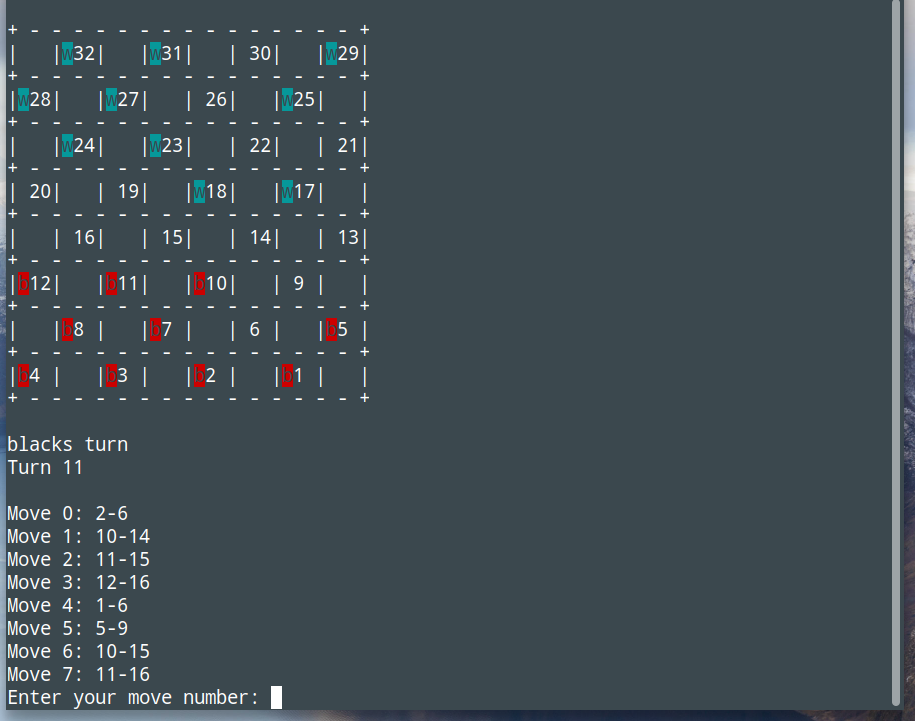
\includegraphics[width=43mm]{cli_humanvsagent.png}
        \vspace{-20pt}
    \end{wrapfigure}

    As our primary intention is to find an agent that learns to play, creating a relatively friendly user interface is not necessarily important, i.e. a simple text-based interface would suffice. Due to the inherent computational strain the project requires, an interface based around a command-line interface (CLI) is to be used. This allows the system to initiate faster than GUIs (Graphical User Interfaces). CLIs reduces the need for package dependencies, configurations and set-ups opposed to GUIs. The simulation would show statistics such as estimated finishing times, current generation count, scores of players in a given generation and the cumulative score of progress of the system.

    When it comes to humans playing against the agent, the checkerboard can also be rendered using ASCII plaintext, users can make inputs through text (in the console or terminal); where the game will show human users the possible moves that a person can take. This system will be used to play against the agent, where the human will take inputs the moves on behalf of the agent's online opponent. A possible rendition is shown in figure \ref{cli_human_input}.


\subsection*{Testing and Evaluation}

    At the end of a given generation, we measure growth of performance by using the generation's champion. Presently we will use the mean of means approach. When a new champion is generated, it is played against the previous 5 champions from earlier generations. 6 games are played for each previous champion, with 3 being as Black, and 3 being White. A mean score is calculated from those 6 games. The overall performance of the current champion is the mean of the 5 sets of games. A positive improvement is when the mean of means are greater than 0. 

    Point Score for the champion games are measured by {1,0,-1} where a Win counts as 1 point and -1 for a loss. The weights are scaled differently to the regular tournament in order to accurately portray the difference between previous champions.

    \subsubsection*{Evaluation Method}

    At the end of the generation run, the end player will be used to compete against human players on various online multi-player checkers websites in order to determine an accurate ELO rating of the system.

    The end player is also used to create comparison games. This player is tested against an agent who is choosing random moves, an agent who is using pure monte-carlo tree searches, and an agent from half the generations generations prior to its current state. These statistics will be used as evidence in order to determine whether the agent is learning, and can also be seriously considered as a viable alternative to other machine learning training approaches.
    % --------------------------------

% Presents the proposed solution(s)
% The design details should all be placed in this section
% Create a number of subsections, each focusing on one issue
% - Make it as clear as possible what you are planning to do
% - But not as a list of steps

% Writing skills (10%)
% • Clarity of presentation of ideas
% • Conformance to paper format standards as specified in Paper Template
% • Quality of writing(readability, grammar)
% • References

% Mark Scheme
% • Adequacy of the proposed solution
% • Specification and design
% • Identification of requirements
% • Description of tools used
% • Overview of architecture
% • Description of lifecycle

% ----------------
% Add references

\bibliography{zotero}

% The list of cited references should appear at the end of the report, ordered alphabetically by the surnames of the first authors.  The default style for references cited in the main text is the  Harvard (author, date) format.  When citing a section in a book, please give the relevant page numbers, as in \cite[p293]{budgen}.  When citing, where there are either one or two authors, use the names, but if there are more than two, give the first one and use ``et al.'' as in  , except where this would be ambiguous, in which case use all author names.

% You need to give all authors' names in each reference.  Do not use ``et al.'' unless there are more than five authors.  Papers that have not been published should be cited as ``unpublished'' \cite{euther}.  Papers that have been submitted or accepted for publication should be cited as ``submitted for publication'' as in \cite{futher} .  You can also cite using just the year when the author's name appears in the text, as in ``but according to Futher \citeyear{futher}, we \dots''.  Where an authors has more than one publication in a year, add `a', `b' etc. after the year..

\end{document}
